% Document body
	%Purpose of tech, derived from tech, example usage, projects that use.
	%Critical thinking, research, comparison to other tech
\section{Network Interfaces}

	\subsection{Overview and Criteria}
	Version 2.0 of the RGB LED Planter Box begins the with the requirements that a web interface be developed for the controller.
	This web interface will hosted on the local controller (localhost), and only this controller will be accessible to it.
	This is true, only if there isn't a network infrastructure to allow this host to share its web interface to other devices.
	This network infrastructure must accomodate the web interface host, other clients wishing to interact with the LED array, and
	be as simple to setup and maintain as possible.  \\

	There are many different types of devices and protocols that allow devices to pass information to each other, and share resources.
	Some of these have become more prominent over time due to adaptation and adoption by the majority of industries worldwide.
	Most devices that need to share resources, do so within local limited bounds of an organization.
	Our web interface ideally should be accessible via a LAN or \textbf{L}ocal \textbf{A}rea \textbf{N}etwork.
	LANs connect computers, servers, printers, and embedded devices in a limited space such as a home, school, or office building. \cite{LAN1}
	However, the choice made should leave room to expand, allowing the web interface to be accessible outside the LAN, if the user is able to provide the necessary resources.

	\subsection{Potential Candidates}
	During our research our team has found three commonly used LAN implementations that fit our project's needs.
	The first is a star topology LAN Over Wire, the second is a star topology LAN over wireless radio, and finally a mesh topology LAN over wireless radio.

	\subsubsection{Star Topology LAN Over Wire}
	Most LANs are based on a star topology.  In this configuration, all end nodes, referred to as clients, are connected to a central hub, which is often a high speed router or switch.
	Each client is connected to the hub via a cable, which is almost always a twisted pair cable.\cite{LAN2}
	In this architecture, all clients are able to communicate to each other by passing their network traffic through the central router.

	\begin{center}
		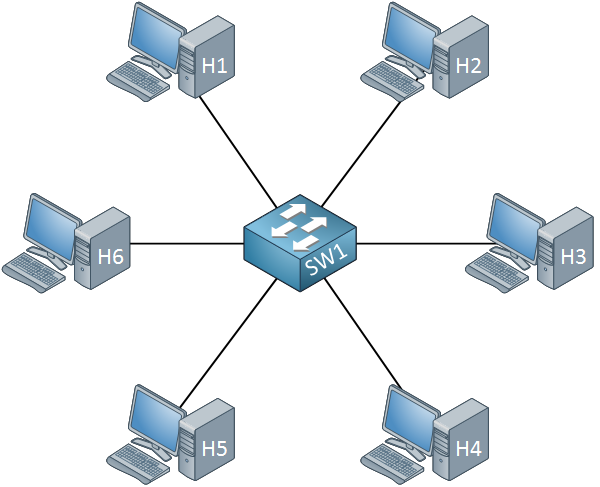
\includegraphics[scale=0.5]{switch-star-topology-hosts.png}
	\end{center} \cite{IMG1}

	\newpage % A better place to break and transition to new page

	\noindent \\ \textbf{Advantages} of using Wire Based Star Topology LANs:
	\begin{itemize}
		\item Traffic sent over wire is guaranteed to reach the destination node, provided the hardware is available.  Having a static physical medium to transfer data across means no data loss.
		\item Connecting new nodes to the network is seamless with IP protocols like DHCP (Dynamic Host Configuration Protocol).
		\item Traffic speed is not inhibited by environmental structure of surrounding area.  As long as the wire connects, one has a constant connection speed.
		\item A single client could fail, but others may continue to communicate on the network due to the architecture.
	\end{itemize}

	\noindent \\ \textbf{Disadvantages} of using Wire Based Star Topology LANs:
	\begin{itemize}
		\item The network infrastructure requires a decent amount of hardware.  Each client that wants to connect needs a wire.
		\item Since all traffic is mediated by a central hub:
		\begin{itemize}
			\item If the hub fails, no clients may communicate with each other or the web interface host.
			\item The hub could become a bottleneck for all network resources under heavy traffic.
		\end{itemize}
	\end{itemize}

	\subsubsection{Star Topology LAN Over Radio}
	This LAN type is nearly the exact same as the wired version, except that clients connect to a hub via wireless radio protocols rather than a cable.
	Standards like IEEE-802.11 allow devices to communicate over radio waves on specific frequencies to pass information to each other.\cite{LAN3}

	\noindent \\ \textbf{Advantages} of using Wireless Radio Based Star Topology LANs:
	\begin{itemize}
		\item Network infrastructure doesn't require much hardware.  Clients and hub need adapters to communicate via radio waves.
		\item Clients can move around freely, and aren't tied down by fixed length cables.  Cables can also physically get in the way.
	\end{itemize}

	\noindent \\ \textbf{Disadvantages} of using Wireless Radio Based Star Topology LANs:
	\begin{itemize}
		\item Wireless radios have to convert wireless signals into understandable frames, and could be slower than wired due to conversion
		\item Radio waves behave like light waves, in that physical objects like walls, can impede the transmission of data.  Data transmission is not guaranteed in every case.
		\item Radios can only handle so many clients transmitting and receiving on a single antennae. Enough clients could slow down a wireless hub.
		\item Disadvantages listed after the first item in \textbf{Star Topology LAN Over Wire}
	\end{itemize}


	\subsubsection{Mesh Topology LAN Over Radio}
	Similar to the \textbf{Star Topology LAN Over Radio}, clients on this network type use wireless radio transmissions to communicate.
	However, in this network architecture, clients communicate with themselves rather than a central hub, acting as a team to deliver information.
	Clients are aware of their neighbors and the potential routes to deliver information to another client on the network.
	Each node in this network architecture behaves as a router for network traffic.
	A good example would be B.A.T.M.A.N (\textbf{B}etter \textbf{A}pproach \textbf{T}o \textbf{M}obile \textbf{A}d-hoc \textbf{N}etworking).  \cite{LAN4}

	\begin{center}
		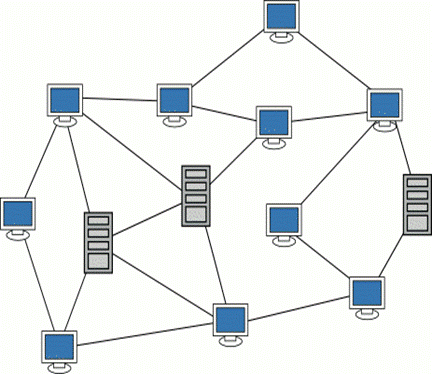
\includegraphics[scale=0.6]{mesh_topology.png}
	\end{center} \cite{IMG2}

	\noindent \\ \textbf{Advantages} of using Mesh Topology LAN Over Radio:
	\begin{itemize}
		\item All advantages listed in \textbf{Star Topology LAN Over Radio}
		\item No single choke point or point of failure in the network
	\end{itemize}

	\noindent \\ \textbf{Disadvantages} of using Mesh Topology LAN Over Radio:
	\begin{itemize}
		\item Taking BATMAN for example, it is relatively new and not in wide-spread use.  Further research is needed into implementation.
		\item Set up time is significantly longer than traditional star topology based networks (must be done manually).
		\item Configuring devices to use this network type along side traditional networks can also be a hassle.
	\end{itemize}


	\subsection{Discussion}
	All of these technologies will connect clients to the hosted web interface, but not all of them meet the criteria for simplicity.
	Using a star architecture, one can eliminate any extra setup time, because most devices are already programmed for "plug n' play" on this topology.
	This topology also allows changes to the network to be made easily and quickly.
	This entire network is not going to be extremely complex either.  The project is not aiming for thousands or even hundreds of clients.
	At a maximum, a distributed system in a greenhouse could be comprised of up to 20 controllable beds, each hosting their own interface.
	(This considers a moderate sized greenhouse found at common private nurseries that sell to the public.) 	The project has envisioned multiple levels of systems,
	but none of these levels cannot be achieved by the simplest of the three network types.  All three could handle every requirement, except simplicity in some cases.

	\subsection{Conclusion}
	Due to the need for simplicity of setup, a star type topology is going to be the network architecture used.
	Because most network infrastructure devices can integrate both wired and wireless device, the end network may see a mix of wireless and wired clients.
	For iteration beginnings and the need for even further simplicity to develop on, the team will most likely start with wired connections.



\section{Custom Enclosure Design}

	\subsection{Overview and Criteria}
	Looking further forward and at further research, vertical lighting and a custom enclosure provide even better growing conditions for the plants.  The enclosure should
	be able to house the plants, soil, the main controller, a slave microcontroller, and the ramparts or verticals that would hold the LED strips.  Still conforming to the
	requirements of simplicity, the design must be affordable, and quick to acquire.  The design must also be able to change as the user sees fit, due to possibly changing
	conditions such as different plants and placement of the enclosure.

	\subsection{Potential Candidates}
	Because there are many options when designing something mechanical in nature, the following options were produced because of their popularity and widespread use.  The
	first option the team explored was 3D printing the necessary hardware for the enclosure.  The second option was simply finding and recommending, or ourselves designing
	pre-fabricated parts to make up the planter beds, that the end user could purchase.  The third option considered was a design involving temporary adhesive connections.

	\subsubsection{3D Printed Hardware}
	In the past few years, 3D printing has exploded as a hobby, and as a practical manufacturing technique for quick, impromptu, custom hardware.  3D printing involves 3D
	generation and rendering of 3d objects in modeling software.  The files created by such modeling software can then be printed.  The printing process involves a printer
	head that moves in the X and Y dimensions, and a printing table that moves up and down in the Z dimesions.  Most printers print a rigid plastic that is heated to
	melting temperatures, and then laid down on the printer table to form layers that make up the 3D object.

	\begin{center}
		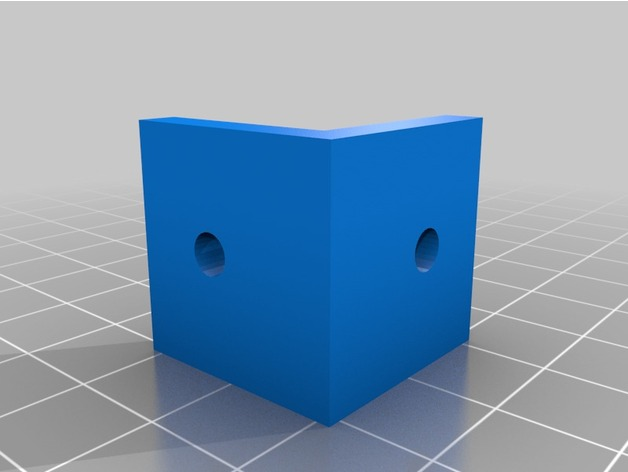
\includegraphics[scale=0.5]{90-degree-bracket.jpg}
	\end{center} \cite{IMG3}

	\noindent \\ \textbf{Advantages} of 3D printing parts for a planter bed:
	\begin{itemize}
		\item Relatively inexpensive compared to other methods or purchasing hardware
		\item If source files provided, 3D printing allows end users to customize the hardware if necessary
		\item Could potentially be quicker to print ones own custom parts, rather than custom order them
	\end{itemize}

	\noindent \\ \textbf{Disadvantages} of 3D printing parts for a planter bed:
	\begin{itemize}
		\item The client might have to learn how to use a 3D printer and 3D modeler, adding complexity.
		\item Hardware may not be printed correctly or could be not as strong as something professionally manufactured.
		\item Hardware may take some a long time to print, depending on what is printed
	\end{itemize}

	\newpage % A better place to break and transition to new page

	\subsubsection{Pre-Fabricated}
	If one is not able to create their own hardware for the planter box, then they might look to someone or a company that could.  Thus, an external source is
	required to make the parts for the end users to most likely purchase.  These pieces of hardware would be professionally created, and often free from
	defect.  The team would be able to recommend parts to the end user, and prepare a simple setup guide to follow to assemble the manufactured parts.

	\noindent \\ \textbf{Advantages} of Pre-Fabricating Parts:
	\begin{itemize}
		\item Client sets up the beds with a simple guide
		\item Client doesn't have to wait on parts to be made
		\item Client doesn't have to make their own parts
	\end{itemize}

	\noindent \\ \textbf{Disadvantages} of Pre-Fabricating Parts:
	\begin{itemize}
		\item Client may not be able to customize the parts to a custom enclosure of their own
		\item Client could end up paying more than other methods
		\item Adds another design implementation to the \textit{software developer's} list (team does not consist of any machinists or mechanical engineers)
	\end{itemize}


	\subsubsection{"Slap On"-type Connections}
	As the name conveys, this option allows one to simply put together parts in a somewhat naïve fashion.  Through the use of adhesive tapes or more structurally sound glues,
	one is able to connect parts by simply putting them face to face, with the adhesive between holding them together.  The adhesive may be a long term hold like epoxy, or a
	short term hold such as two-sided foam tape.

	\noindent \\ \textbf{Advantages} of "Slap On"-type Connections:
	\begin{itemize}
		\item The least expensive option provided.  Easy to get replacements.
		\item The easiest to assemble and disassemble, this option stands out for mobility purposes.
	\end{itemize}

	\noindent \\ \textbf{Disadvantages} of "Slap On"-type Connections:
	\begin{itemize}
		\item "You get what you pay for." Items are not durable.
		\item Connections may not hold permanently or are insecure.  Electrical connections might suffer at this option.
		\item Connections may not hold at all, and planter beds may fall apart depending on weight forces.
	\end{itemize}


	\subsection{Discussion}
	Seeing that this section doesn't quite have a coding or electical design to it, not much time was spent on developing options.  The options considered were found to be the
	simplest.  Of the three, the least cost and effort would go towards the "Slap-On" method.  However cheap and easy it may be, this option may prove not to have the structural
	integrity that the application requires.  Designing parts to have fabricated is an option that likely would not be implemented, but it is not out of the question.  This option
	adds an exteme layer of simplicity for the end user, who would basically have to follow a simple instruction set to assemble said parts.  However, the team doesn't have a
	mechanical or civil engineering background, and further research or collaboration with outside sources would be required to complete this implementation.  The last option of
	3D printing the parts necessary offers the argument of being simple to produce, relatively inexpensive, and customizable.

	\subsection{Conclusion}
	Due to the factors that the enclosure must be simple to create and modify, the team has opted to use 3D printed parts as the viable solution.  This is because of current knowledge
	levels of the team to be able to manufacture parts, the simplicity of the method, and the increasing reliability of 3D printers.  This option also features the structurally integrity
	that the planter box will require.  Since this section is part of the stretch goals of the project, simplicity and cost force the choice of this option.

	\newpage % A better place to break and transition to new page

	\section{Control Service Language}

		\subsection{Overview and Criteria}
		The Control Service will be the main program that interfaces between the Web Interface and the microcontrollers driving the RGB LEDs.  It doesn't necessarily need to be simple
		for the end user, since they may not ever need to interact with it.  However, it should be simple enough for the team to understand, so that development and bug squashing comes
		easier.  The language that the Control Service is written in, will play a crucial part in development and testing.  This language is also restricted to the particular hardware
		that will be used in the project.  If a Raspberry Pi is used as the main microcontroller, it will not be able to run languages that are process or memory intensive.

		\subsection{Potential Candidates}
		Heavily based upon the restrictions of hardware, the team has selected the following programming languages.  The first option is the widely used and persistent C/C++ language.
		The second option considered was a language that closely mimics the language used to write the web interface control.  The third and final option was Rust, a new member of the
		C++ family.

		\subsubsection{C/C++}
		The C language has been around since the early 1970s. \cite{LANG1}  It is extremely powerful compared to other languages because it is one of the few languages that comes closely
		to mimicing Assembly, a very low level microprocessor instruction language.  This means that when compiled, the code produces an efficient executing program.  Efficient in the terms
		that the processor can do the most in the least amount of time, with the least amount of memory. Considering these ideologies, the UNIX and *nix family of operating systems
		foundations are built on this language.  From C sprouted C++, which essentially is the same core language.  The only difference between the two is that C++ was developed to support Object Oriented (OO) programming.  C++ programming has the caveats of
		being based on the C language while incorporating the powerful idea of objects in a programming language.

		\noindent \\ \textbf{Advantages} of using C/C++:
		\begin{itemize}
			\item Extremely fast execution
			\item Lightweight in memory
			\item Small and efficient enough to run on the most basic microprocessors
			\item The team is already familiar with the language due to previous use
			\item The LED strips and their already developed libraries are based on C/C++
			\item Documentation and examples for these languages are nearly endless
		\end{itemize}

		\noindent \\ \textbf{Disadvantages} of using C/C++:
		\begin{itemize}
			\item The language is somewhat restrictive on syntax and operation
		\end{itemize}


		\subsubsection{Web Based Language(NodeJS, PHP, etc)}
		Considering that the main front facing interface between the user and the LEDs will be a Web Interface, the language that this interface is written in must be considered to operate
		the Control Service.  NodeJS or PHP would be two choices for the language selected to drive the front end.

		\noindent \\ \textbf{Advantages} of using Web Based Language:
		\begin{itemize}
			\item Front end that the user sees is written in the same languages
			\item Reduces number of languages used through the project
		\end{itemize}

		\noindent \\ \textbf{Disadvantages} of using Web Based Language:
		\begin{itemize}
			\item Interfacing with the microcontoller driving the LEDs would be extremely difficult (most Web languages never have to pass serial to a microcontoller)
			\item The language may not have the proper process control compared to languages that drive operating systems or other small microcontrollers
			\item The language may not run efficiently on the smaller microcontroller when trying to perform the necessary operations of the Control Service.
		\end{itemize}


		\subsubsection{Rust}
		A relatively new language, Rust is basically a child of C++.  While being syntactically very similar to C++, Rust claims to have better memory managment, and also be developed with the
		sense that the language should maintain system functionality.  Rust has grown to be a new choice for operating systems, game engines, and even virtual reality applications. \cite{LANG2}

		\noindent \\ \textbf{Advantages} of using Rust:
		\begin{itemize}
			\item Light on memory and processing
			\item Newer language means potential for new features, specifically object controller
			\item Lots of documentation on the language
		\end{itemize}

		\noindent \\ \textbf{Disadvantages} of using Rust:
		\begin{itemize}
			\item Being a relatively new language, the team has not had experience with it.
			\item For the same reason above, the documentation specific to the project application or its hardware may not exist.
			\item Rust does have very strict coding practices, that may not be enforceable on the selected hardware.
		\end{itemize}


		\subsection{Discussion}
		Looking further into the requirements for the project, the LED strips have to be driven with a library of some sort that has been developed with C or C++.  Thus, being written in a OS
		type language, the team should be able to implement the same features or applications of the libraries into the Control Service.  C/C++ is also very efficient compared to NodeJS or PHP.
		These specific Web languages also do not have the immediate capabilities to interface with a microcontroller to update the LEDs.  Rust does have its caveats in being new and efficient
		at the same time, but adaptation and adoption of this new language might prove challenging while a simpler solution exists.

		\subsection{Conclusion}
		The team has selected C++ to be the lead language in the Control Service.  It's relativeness to the LED libraries that drive the hardware, combined with the team's knowledge on it and
		the efficiency of the language, it presents itself as the clear front runner.  It clearly meets every requirement laid out by the team, and currently has too little drawbacks to be replaced
		by another of the proposed languages.
